\section{Experiments}
\label{sec:experiments}
\subsection{Protocol and comparison scope}
HotpotQA distractor evaluation used supplied question contexts
\citep{yang2018hotpotqa}: 150 hard training questions, 300 disjoint hard
validation questions, and 300 hard primary test questions. Training and
validation came from the official training split; primary test used the
official validation split. Search adjusted allocation, not model weights.
Five paired seeds $\{11,23,37,53,71\}$ and actual search-cost cutoffs of
16M, 24M and 32M covered eleven methods.

The common one-round RAG grammar contained 61,344 syntactic workflows.
Eight root query actions comprised identity, document generation, two
Query2doc mixtures~\citep{wang2023query2doc}, decomposition, rewriting,
synonymous rewriting and HyDE~\citep{gao2023hyde}. Retrieval, fusion,
evidence selection, reranking, width and ordering completed each workflow.
Generated retrieval passages were never answer evidence. Qwen3.5-4B served
all generative roles~\citep{qwen2026qwen35}; E5-base-v2, BGE-M3 and
Qwen3-Embedding-0.6B supplied encodings
\citep{wang2022e5,chen2024bgem3,zhang2025qwenembedding}.

Each trial owned a private cache. The four original MCTS allocators shared
eight-root initialization, uniform expansion and rollout,
raw-return backup and the same execution service. MCTS-Random chose children
uniformly; uniform-terminal search instead sampled whole workflows.
All 150 training outcomes joined before one mean-F1 backup, price update
or next tree decision, even when four queries executed together.
The MCTS coefficient was $c=1.4$, with $\beta=2$ for both cost-aware rules
and independently calibrated $C_{\rm ref}\approx1.471$M weighted tokens
(the exact frozen value is retained in the supplement).
Greedy bfloat16 generation used fixed groups of at most four.

At each cutoff, the up to five distinct completed workflows ranked highest
by training F1 entered validation. Validation F1 selected one endpoint;
ties followed fixed training order. Test outcomes never selected workflows
or updated allocation. The primary outcome was validation-selected test F1.
Auxiliary EM, per-seed quality, component choices, all phase bills, adapter
details and inference settings are in the supplement.

\paragraph{Actual-cost accounting.}
RAG prices weighted each request's actual unpadded input and output tokens
by model parameter count in billions; this proxy is neither GPU time nor
FLOPs. Evaluations completed before actual bills determined the last complete
snapshot at or below a reporting budget. Crossing evaluations remained
billed, and their future rewards and cache state were excluded from earlier
snapshots. The full optimization bill $C_{\rm opt}$ included all search,
crossing work, validation and paid failures or retries. Shared preparation
and primary-test measurement were separate. The auxiliary diagnostic
$J=F-0.05C_{\rm opt}/C_{\rm ref}$ used $F\in[0,1]$ and one full bill per
seed; neither backup nor endpoint selection optimized it.

\paragraph{Controls.}
AgentUCT-StaticFull froze calibrated prices and zero-history continuation
against an empty pricing cache while retaining live execution reuse.
AFlow--RAG preserved its Top4 score/uniform parent mixture and charged
Qwen proposals and repairs. FLASH*--RAG used D-optimal design, linear EIPS
and categorical TPE; EEIPU combined objective and stage-cost GPs with cached
prefix proposals; LaMBO used slowly moving regions and local GP-UCB; MSBO
used cascade start/advance decisions and full-panel feedback barriers.
Their initializations and declared adapters remained part of each policy.
LaMBO's switching-cost helper was unused, so its native regret guarantee
was not transferred. These comparisons evaluate allocation within a common
system, not reproduction of each source paper's benchmark or cache policy.

\subsection{Quality at matched RAG budgets}
\label{sec:stage-results}
AgentUCT had the highest mean at 32M among the eleven compared methods
(Table~\ref{tab:direct-algorithm-coverage}; Figure~\ref{fig:budget-quality}).
Its $69.57\pm0.28\%$ mean test F1 exceeded MCTS-UCT's $68.01\pm1.12\%$
by 1.56 percentage points. All five paired test-score differences were
positive; the seed-11 endpoints were identical and their 0.067-point
difference arose from fresh numerical execution variation. Common evaluator
settings therefore do not establish the fixed-table assumption empirically.

\begin{table}[t]
\centering\small
\caption{Direct RAG test F1 at 32M weighted-token search cost, mean $\pm$
sample SD across five paired seeds. All rows share validation selection and
the test panel. All budgets and seeds remain in the supplementary tables.}
\label{tab:direct-algorithm-coverage}
\begin{tabular}{lr}
\toprule
Method & Test F1 (\%)\\
\midrule
AgentUCT & $69.57\pm0.28$\\
MCTS-UCT & $68.01\pm1.12$\\
AgentUCT-NextC & $68.22\pm1.96$\\
AgentUCT-StaticFull & $67.36\pm2.67$\\
MCTS-Random & $68.80\pm0.87$\\
AFlow--RAG & $67.25\pm1.57$\\
FLASH*--RAG (TPE) & $67.29\pm0.85$\\
EEIPU--RAG & $67.29\pm0.78$\\
LaMBO--RAG & $66.11\pm2.62$\\
MSBO--RAG & $67.44\pm2.53$\\
Uniform-terminal & $67.18\pm1.59$\\
\bottomrule
\end{tabular}
\end{table}

The higher mean did not require more completed evaluations: AgentUCT
retained 17.6 on average, against MCTS-UCT's 17.8 and AFlow's 21.0.
Across the original four MCTS methods, all 214 recorded adaptive RAG
selections occurred at the root, followed by uniform expansion and rollout.
Within AgentUCT's retained 32M prefixes,
the cost term changed 28 of 48 choices relative to maximizing the saved
$Q+\mathrm{bonus}$ at the same state. One seed-53 decision gave up 0.0353
quality-index units for a predicted 0.760M reduction in complete cost.
Saved scores establish changed allocation without reconstructing forecasts
or assigning a test-score gain to an individual action.

At 16M, the four original MCTS methods selected the same workflow per seed.
Eight-root initialization cost 12.287--16.626M, and only seed 23 retained
adaptive completions at that cutoff. Within each AgentUCT and MCTS-UCT run, the 24M and 32M snapshots reused
that run's endpoint and complete test measurement. These cutoffs provide
five endpoint comparisons, not ten independent repeats.
The curves do not establish an optimal stopping budget.

\begin{figure*}[t]
\centering
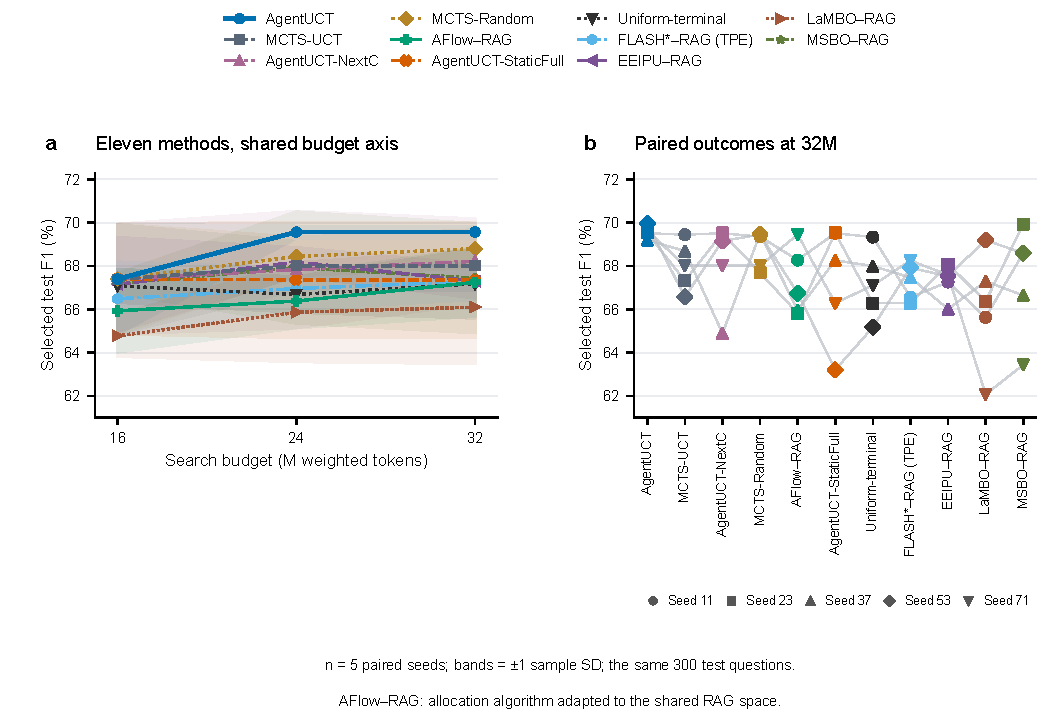
\includegraphics[width=0.96\textwidth]{figures/rag-budget-overlay-20261004/five-seed-budget-overlay.pdf}
\caption{Test F1 after validation selection at actual search-cost cutoffs.
(a) Eleven method means and $\pm$ one sample SD across five paired seeds
share axes. (b) Every paired 32M outcome. Endpoint reuse creates correlated
budget measurements; smaller-budget and seed-level reversals are retained.}
\Description{Eleven methods share test F1 versus actual search budget axes with sample SD bands. A second panel retains all matched seed outcomes at 32 million weighted-token units.}
\label{fig:budget-quality}
\end{figure*}

AgentUCT led AFlow in all seeds at 24M and 32M, and uniform-terminal,
FLASH*, EEIPU and LaMBO in all seeds at 32M. MSBO led in seed 23 by
0.41 points. At 16M, all five sampling/surrogate/stage controls exceeded
AgentUCT in seed 53; LaMBO led by 0.39 points in seed 37 at 24M.
Thus the highest 32M mean is specific to this cohort and does not describe
every seed or budget. Fifty prespecified random workflows reached
$60.58\pm5.22\%$ mean F1 (workflow SD), median $62.11\%$; three fixed
Query2doc--BM25, HyDE--E5 and RankGPT-style adaptations~\citep{sun2023rankgpt} reached 61.60,
62.89 and 62.53\%. All fifty draws, rather than a test-best subset, entered
the reference distribution.

\subsection{Estimator and endpoint-selection ablations}
\label{sec:skip-validation}
AgentUCT's advantage over MCTS-UCT persisted without validation. On the same retained
searches, direct testing of the highest training-F1 workflow gave AgentUCT
$69.24\pm0.74\%$ and MCTS-UCT $67.37\pm0.53\%$ at 32M, with paired
gain $1.87\pm1.24$ points. The supplement retains all sixty training-Top1
method--seed--budget cells. Test outcomes never selected a workflow or
changed a snapshot.

\paragraph{Estimator adaptation.}
\label{sec:static-full-results}
Full suffix pricing exceeded AgentUCT-NextC's mean by 1.73 points at 24M
and 1.35 at 32M; at 32M, three seeds improved and two tied. Direct
training-Top1 selection reduced this gap to 0.35 points. Against
AgentUCT-StaticFull, AgentUCT's paired 32M difference was
$2.21\pm2.89$ points: three gains and two ties, with identical retained
evaluation counts per pair. These interventions support complete-cost
pricing and joint estimator adaptation in this protocol; the static
comparison does not separate cache conditioning, price learning and demand.

Higher F1 did not imply higher full-bill utility. AgentUCT's mean
$C_{\rm opt}$ was 59.003M, compared with MCTS-UCT's 59.624M and
AgentUCT-NextC's 58.319M. Its mean $J$ was 0.03670 above MCTS-UCT and
0.00978 below AgentUCT-NextC, chiefly because of validation cost.
Logical hit rates at 32M were 6.79\% for AgentUCT and 6.81\% for MCTS-UCT.
These paths have different workloads; no matched cache-disabled speedup was
measured. Every saved RAG prefix covered all training queries, placing this
experiment in the exactly compressible full-panel graph case.

\subsection{Generated workflows on GSM8K}
GSM8K~\citep{cobbe2021verifiers} used five paired seeds and panels of 150 training, 300 validation and
300 primary test questions. AgentUCT and MCTS-UCT shared Qwen3.5-4B,
fixed-eight groups, Python operators, proposer/repair settings, counted-error
histories, progressive widening $\min(8,\max(1,\lceil\sqrt N\rceil))$, depth limit
12 and no rollout. They differed in completion pricing. AFlow retained its
Top4 parent policy in the same adaptation. Independent fixed-path cost
calibration froze $C_{\rm ref}=150{,}954.5$ raw tokens and budgets of
6.423M, 12.772M and 19.122M; test quality did not enter calibration.
Up to five training-ranked completed workflows entered validation per snapshot.

\begin{table*}[t]
\centering\small
\caption{Complete GSM8K accuracy (\%), mean $\pm$ sample SD across five
paired seeds at raw-token budgets 6.423/12.772/19.122M. Rows report original
method scores; SD is not a confidence interval.}
\label{tab:generated-complete-main}
\begin{tabular}{llrrr}
\toprule
Task & Method & First & Middle & Largest\\
\midrule
GSM8K & AgentUCT & $93.07\pm1.52$ & $93.00\pm1.49$ & $93.07\pm1.48$\\
 & MCTS-UCT & $92.60\pm1.09$ & $92.60\pm0.86$ & $92.67\pm0.78$\\
 & AFlow & $91.60\pm1.95$ & $92.93\pm1.26$ & $93.07\pm1.40$\\
\bottomrule
\end{tabular}
\end{table*}

At the largest GSM8K cutoff, AgentUCT led MCTS-UCT in three seeds, tied
in one and trailed in one. Its $93.07\%$ mean was exactly equal to AFlow's
before rounding (Table~\ref{tab:generated-complete-main}). Saved traversals
show recursive cost-induced choices; a recorded depth-one choice yielded
zero training score, while AgentUCT seed 71 selected initial node 0 at all
three budgets. Decision evidence therefore does not attribute endpoint
accuracy gains to those particular choices.

The supplement retains all 45 GSM8K quality cells, equally
weighted seed means, sample SDs with denominator $n-1$, and full actual
ledgers. Common questions and repeated endpoints correlate budgets.
Physical failures, candidate errors, repair calls and whole crossing
evaluations remain scored or billed under their original protocols;
overshoot is a subset of the bill, not an extra charge. GSM shared
preparation cost 109,983 raw tokens is a separate one-time item. These raw-token costs remain distinct
from RAG's model-weighted units. Retired proposal-history cohorts and
the earlier bounded pilot do not enter this complete comparison.
